\chapter{Evaluation}
\label{chap:evaluation}

% compare:
% - mono (no best fuzzer for sample programs)
% - multi vs single (more communication is better if multi > single)
% - coop vs union (test coop efficacy)

This chapter presents an evaluation of four different fuzzers and our
implementation of the \acf{CFF} as described in Section~\ref{sec:system-impl};
the implementation uses the same four fuzzers in order to draw meaningful
comparison results.

\paragraph{Choice of Fuzzers}

For the choice of fuzzers we decided to use \aflfast, \fairfuzz, \honggfuzz\@
and \vuzzer. The first two provide two different implementations of the
state-of-the-art \ac{CGF}, \afl; we argue that two different implementation of
the same core algorithm may yield different results. \honggfuzz\@ is chosen as
it provides different means to extract feedback from the \sut, possibly
resulting in a different feedback signal (given the same input) compared to
other methods (\eg\@ \afl\@ uses QEMU). Lastly, \vuzzer\@ provides with an
evolutionary fuzzer which uses static and lightweight program analysis; because
of this, \ac{CFF} uses the congestion control mechanism to interact with
\vuzzer. All fuzzers were run with the default parameters and configuration,
with the exception of those required to correctly interface with the \sut.

\paragraph{Experimental Infrastructure}

Experiments were run on a 64-bit machine with $8$ cores (running at $3.4$GHz),
with $16$GB of RAM, running Ubuntu 16.04. Because of a limitation of \vuzzer\@
implementation, we had to run it inside a virtual machine hosting Ubuntu 14.04.
To allow communication with its driver running on the host machine, we used a
shared folder; this allowed us to reuse the \texttt{inotify} infrastructure as
if the fuzzer was running locally.

\paragraph{Testing Targets}

We chose a set of programs that are widely used both in practice and literature:

\begin{description}
    \item[\djpeg] uses the popular \texttt{libjpeg-turbo} (version 1.5.1) and
        has been used for the evaluation of \fairfuzz\@ and \vuzzer;
    \item[\objdump] is a component of the suite \texttt{binutils} (version 2.28)
        which has also been tested by \aflfast\@ and \fairfuzz; we test it with
        the command line option \texttt{-d}, which provides a disassembler;
    \item[\tiffpdf] from the popular \texttt{libtiff} (version 4.0.9), parses a
        TIFF image and converts it to a PDF\@; we use it without command line
        arguments;
    \item[\listswf] from the popular \texttt{libming} (version 0.4.8), parses a
        file in SWF format; we use it without command line arguments.
\end{description}

Moreover, as \vuzzer\@ requires a minimum set of seed inputs to work properly,
we randomly chose the minimum required by \vuzzer\@ from test samples provided
with each \sut; these inputs were used to also seed other fuzzers.

As an additional information, we report on the number of basic block and
functions found by static analysis via Radare\footnote{\url{https://rada.re/}}
in Table~\ref{tab:eval-bbs}.

\begin{table}[h]
    \centering%
    \begin{tabular}{l c c}
        \textbf{\sut} & \textbf{basic blocks} & \textbf{functions} \\
        \bottomrule%
        \djpeg& $6187$ & $366$ \\
        \objdump& $43211$ & $2220$ \\
        \tiffpdf& $11129$ & $791$ \\
        \listswf& $3349$ & $446$
    \end{tabular}
    \caption{Number of basic blocks and functions for the chosen targets.}
    \label{tab:eval-bbs}
\end{table}

\section{Single Fuzzer Evaluation}
\label{sec:eval-mono}

In this section we present an evaluation of the chosen fuzzers, without any
cooperation. We ran each fuzzer independently for $24$ hours on each of the
targets, except for \listswf\ which ran for $6$ hours.
Table~\ref{tab:eval-mono} reports the arithmetic mean and the $95\%$ confidence
intervals for the number of unique basic block transitions as computed by Intel
\ac{BTS} over five rounds. The coverage values are aggregated over time
intervals of one minute.

\begin{table}[h]
    \centering%
    \small%
    \begin{adjustbox}{tabular=l*{4}c,center}
        \textbf{\sut} & \textbf{\aflfast} & \textbf{\fairfuzz} &
            \textbf{\honggfuzz} & \textbf{\vuzzer} \\
        \bottomrule%
        \djpeg& $3739.4 \pm 113.831$ & $4043.2 \pm 103.838$ &
            \hicell$4112.8 \pm 39.5483$ & $2801 \pm 53.5514$ \\
        \objdump& $4762.6 \pm 23.3693$ & \hicell$5067 \pm 62.6832$ &
            $4132.4 \pm 104.8$ & $3162.2 \pm 138.462$ \\
        \tiffpdf& \hicell$8971.2 \pm 152.865$ & $8813.8 \pm 146.756$ &
            $5260.2 \pm 148.591$ & $3616 \pm 34.6427$ \\
        \listswf& $6831.6 \pm 2615.24$ & \hicell$8586.8 \pm 87.7467$ &
            $6345.6 \pm 2358.52$ & $5048.2 \pm 90.3928$
    \end{adjustbox}
    \caption{Mean coverage with $95\%$ confidence intervals for single fuzzers.
    Highlighted is the best for the given program.}
    \label{tab:eval-mono}
\end{table}

By looking at the table, as well as at Figure~\ref{fig:eval-mono}, which
presents the evolution of coverage over time, it is easy to see how no fuzzer is
decisively better than the others across all tested programs. This validates,
although for a small sample of programs and fuzzers, our intuition based on the
no free lunch theorem, for which there is no fuzzer that performs better than
all others across all possible test programs.

\begin{figure}[h]
    \centering%
    \begin{adjustbox}{center}
        \subfloat[\djpeg]{%
            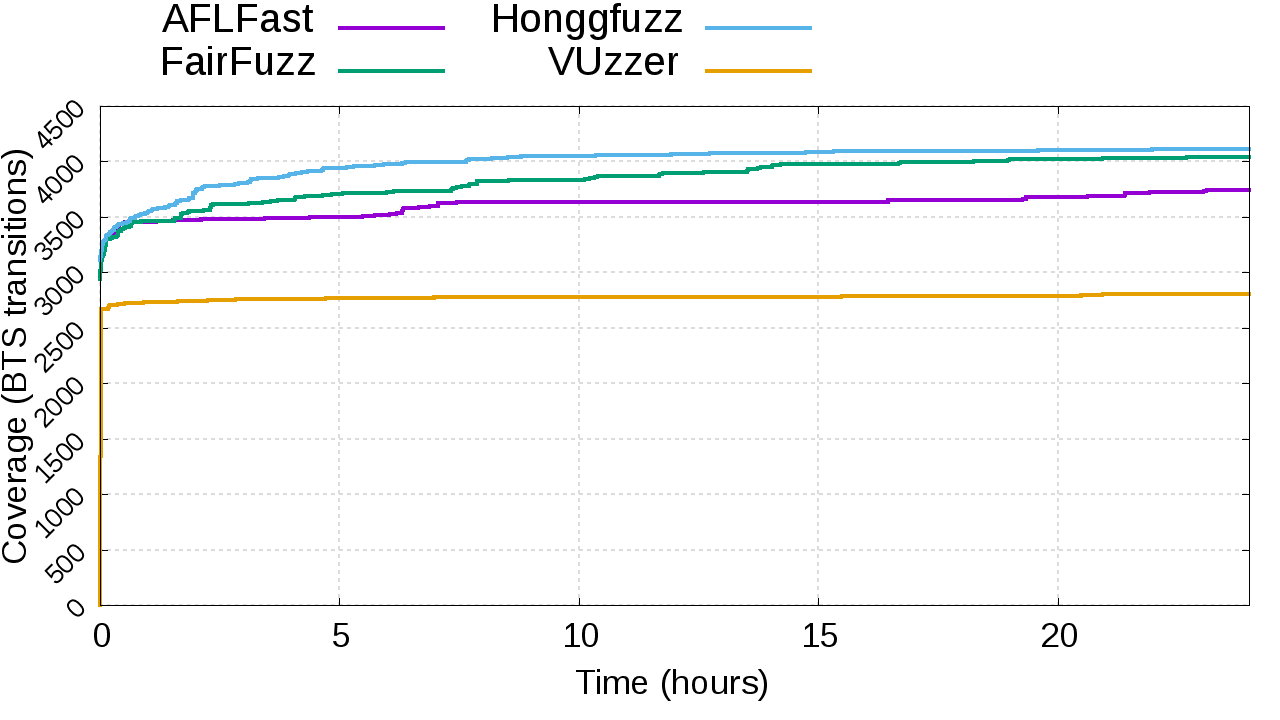
\includegraphics[width=.65\textwidth]{figures/mono-djpeg}
            \label{fig:eval-mono-djpeg}
        }
        \subfloat[\objdump]{%
            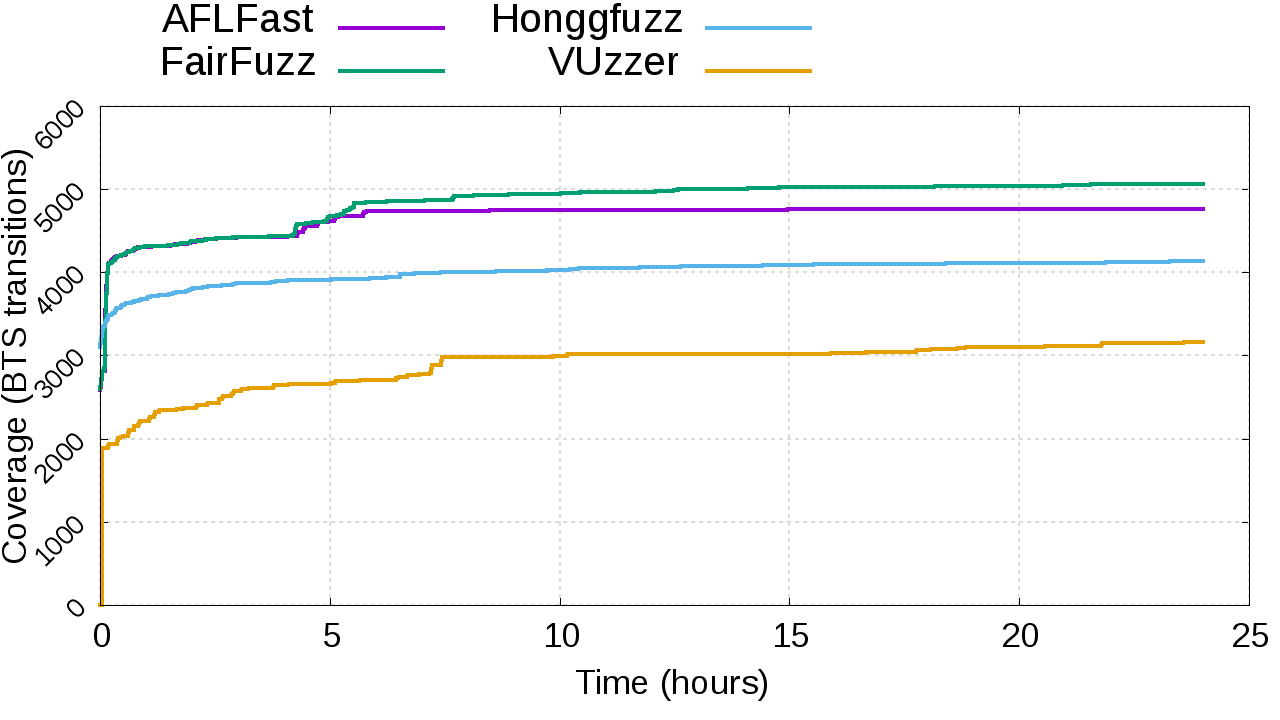
\includegraphics[width=.65\textwidth]{figures/mono-objdump}
            \label{fig:eval-mono-objdump}
        }
    \end{adjustbox}
    \begin{adjustbox}{center}
        \subfloat[\tiffpdf]{%
            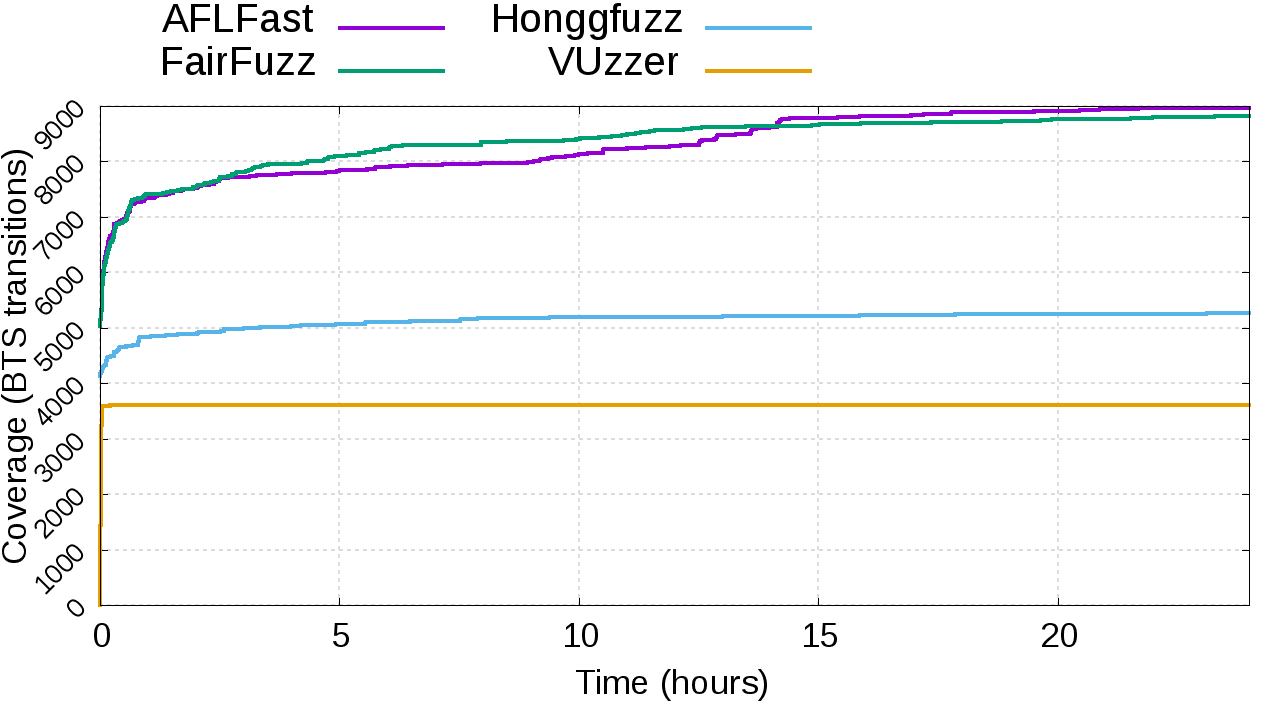
\includegraphics[width=.65\textwidth]{figures/mono-tiff2pdf}
            \label{fig:eval-mono-tiff2pdf}
        }
        \subfloat[\listswf]{%
            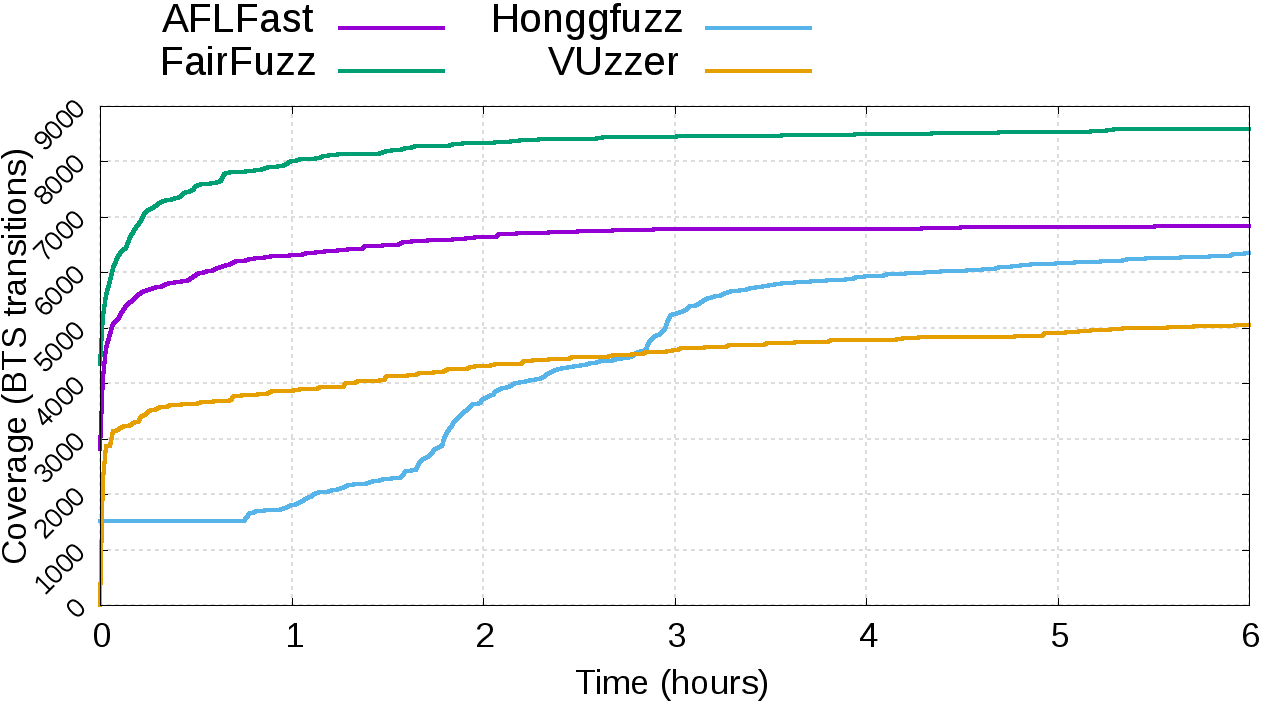
\includegraphics[width=.65\textwidth]{figures/mono-ming}
            \label{fig:eval-mono-ming}
        }
    \end{adjustbox}
    \caption{Mean coverage over time for single fuzzers.}
    \label{fig:eval-mono}
\end{figure}

To derive more robust and meaningful insights over these results, we employ the
Bayesian estimation model proposed in~\cite{kruschke2013bayesian}. This model
provides, among others, estimates of the posterior distributions of the means
and their differences of two given sets of observations.
Figure~\ref{fig:djpeg-means} shows the distribution of the difference of means
of \honggfuzz\ against \aflfast\ and \fairfuzz\ for \djpeg. The figure also
shows the $95\%$ \ac{HDI}, which represents the interval of values onto which
$95\%$ of the probability mass lies. Figure~\ref{fig:djpeg-m-hongg-afl} clearly
shows that the \ac{HDI} lies completely above zero, meaning that with high
credibility we can say that \honggfuzz\ performs better than \aflfast\ over
\djpeg. Unfortunately the same conclusion cannot be made for the comparison of
\honggfuzz\ against \fairfuzz. Figure~\ref{fig:djpeg-m-hongg-fair} shows that a
difference of means of zero lies on the \ac{HDI}; moreover an estimated $20.2\%$
of the probability mass lies below zero (\ie~in favor of \fairfuzz).

\begin{figure}[h]
    \centering%
    \subfloat[\honggfuzz\ vs.\ \aflfast]{%
        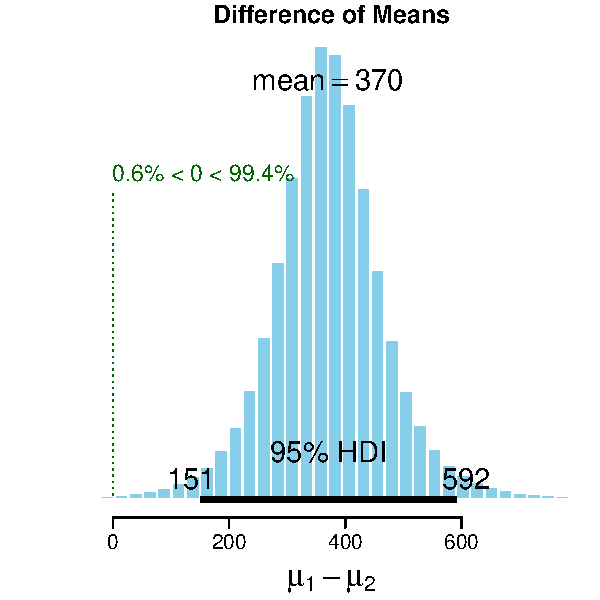
\includegraphics[width=.4\textwidth]{figures/cropped/djpeg-m-hongg-afl}
        \label{fig:djpeg-m-hongg-afl}
    }
    \subfloat[\honggfuzz\ vs.\ \fairfuzz]{%
        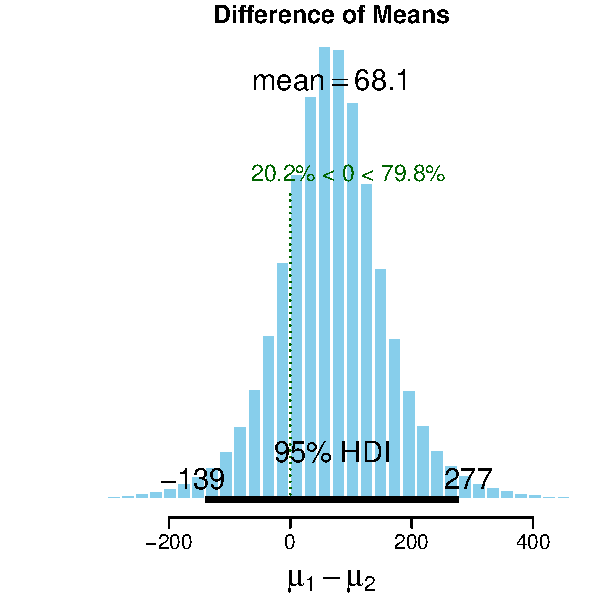
\includegraphics[width=.4\textwidth]{figures/cropped/djpeg-m-hongg-fair}
        \label{fig:djpeg-m-hongg-fair}
    }
    \caption{Single fuzzers: distribution of difference of means for \djpeg.}
    \label{fig:djpeg-means}
\end{figure}

Figure~\ref{fig:objdump-means} shows the difference of means for \objdump. For
both the cases of \fairfuzz\ against \aflfast\
(Figure~\ref{fig:objdump-m-fair-afl}) and \fairfuzz\ against \honggfuzz\
(Figure~\ref{fig:objdump-m-fair-hongg}) the results strongly support the claim
of \fairfuzz\ uncovering more basic block transitions for \objdump.

\begin{figure}[h]
    \centering%
    \subfloat[\fairfuzz\ vs.\ \aflfast]{%
        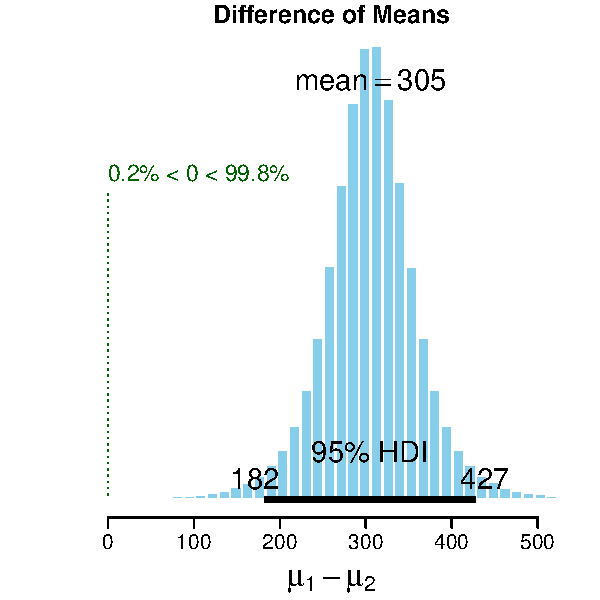
\includegraphics[width=.4\textwidth]{figures/cropped/objdump-m-fair-afl}
        \label{fig:objdump-m-fair-afl}
    }
    \subfloat[\fairfuzz\ vs.\ \honggfuzz]{%
        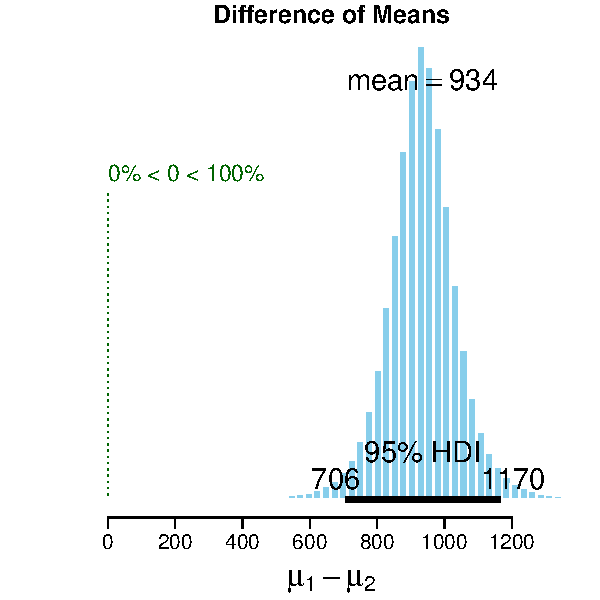
\includegraphics[width=.4\textwidth]{figures/cropped/objdump-m-fair-hongg}
        \label{fig:objdump-m-fair-hongg}
    }
    \caption{Single fuzzers: distribution of difference of means for \objdump.}
    \label{fig:objdump-means}
\end{figure}

Figure~\ref{fig:tiff2pdf-means} shows the difference of means for \tiffpdf.
Unfortunately, as for \djpeg, we are not able to decisively confirm whether
\aflfast\ is better than \fairfuzz\ (Figure~\ref{fig:tiff2pdf-m-afl-fair}). We
can be instead more certain affirming that \aflfast\ outperforms \honggfuzz\ for
the given \sut\ (Figure~\ref{fig:tiff2pdf-m-afl-hongg}).

\begin{figure}[h]
    \centering%
    \subfloat[\aflfast\ vs.\ \fairfuzz]{%
        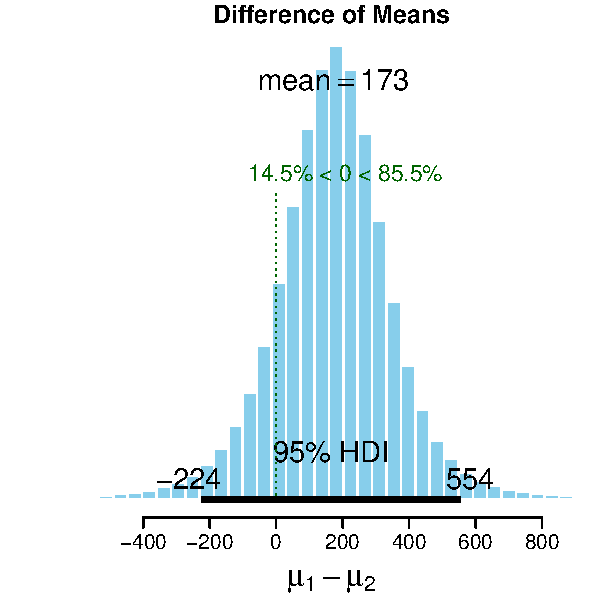
\includegraphics[width=.4\textwidth]{figures/cropped/tiff2pdf-m-afl-fair}
        \label{fig:tiff2pdf-m-afl-fair}
    }
    \subfloat[\aflfast\ vs.\ \honggfuzz]{%
        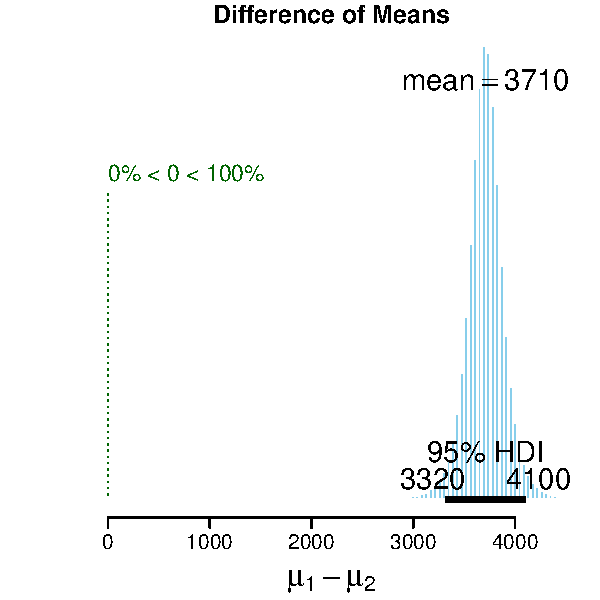
\includegraphics[width=.4\textwidth]{figures/cropped/tiff2pdf-m-afl-hongg}
        \label{fig:tiff2pdf-m-afl-hongg}
    }
    \caption{Single fuzzers: distribution of difference of means for \tiffpdf.}
    \label{fig:tiff2pdf-means}
\end{figure}

To validate differences among fuzzers even further, we compare, in
Table~\ref{tab:eval-mono-union}, the best single fuzzer with the result of
taking the union of coverage traces across all four fuzzers for each time step.
The table clearly shows that fuzzers uncover unique basic block transitions that
are not exposed by any other fuzzer (\ie~uncover disjoint sets of transitions)
and this contributes to reaching an higher final coverage consistently across
all examined programs.

\begin{table}[h]
    \centering%
    \begin{tabular}{l c l c}
        \textbf{\sut} & \multicolumn{2}{c}{\textbf{best single}} & \textbf{union} \\
        \bottomrule%
        \djpeg& $4112.8 \pm 39.5476$ & \honggfuzz& \hicell$4157.2 \pm 40.0495$ \\
        \objdump& $5067 \pm 62.6821$ & \fairfuzz& \hicell$5404.6 \pm 38.1997$ \\
        \tiffpdf& $8971.2 \pm 152.8626$ & \aflfast& \hicell$9695 \pm 129.7239$ \\
        \listswf& $8586.8 \pm 87.7451$ & \fairfuzz& \hicell$8916.6 \pm 83.8365$
    \end{tabular}
    \caption{Mean coverage with $95\%$ confidence intervals for best single
    fuzzer and union of coverage traces.}
    \label{tab:eval-mono-union}
\end{table}

To delve deeper into these values, we show the result of Bayesian estimation in
Figure~\ref{fig:means-mono-union}. The $95\%$ \ac{HDI} falls above zero (\ie~in
favour of the union of fuzzers) for all considered programs except \djpeg, for
which the results are inconclusive.

\begin{figure}[h]
    \centering%
    \subfloat[\djpeg: Union vs.\ \honggfuzz]{%
        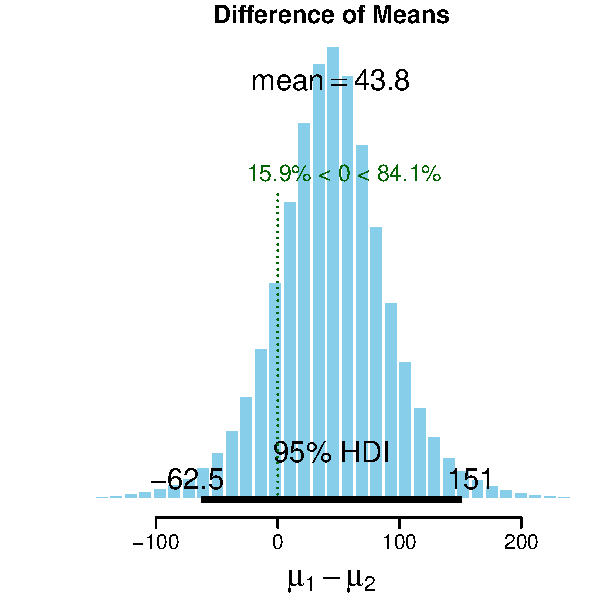
\includegraphics[width=.4\textwidth]{figures/cropped/djpeg-m-uni-hongg}
    }
    \subfloat[\objdump: Union vs.\ \fairfuzz]{%
        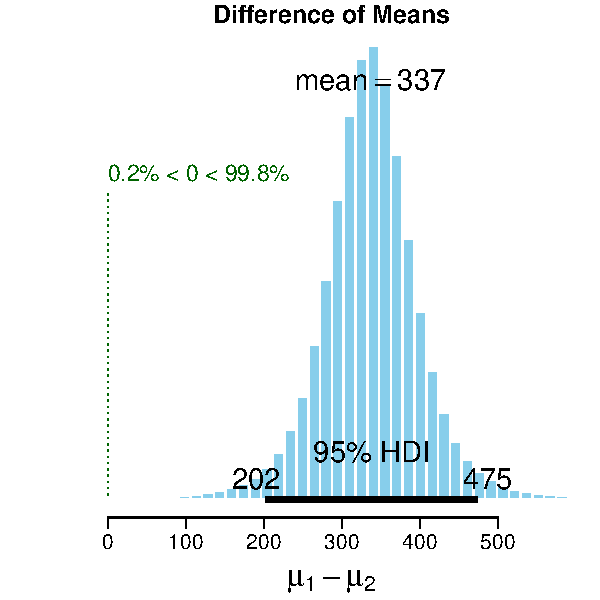
\includegraphics[width=.4\textwidth]{figures/cropped/objdump-m-uni-fair}
    }\\
    \subfloat[\tiffpdf: Union vs.\ \aflfast]{%
        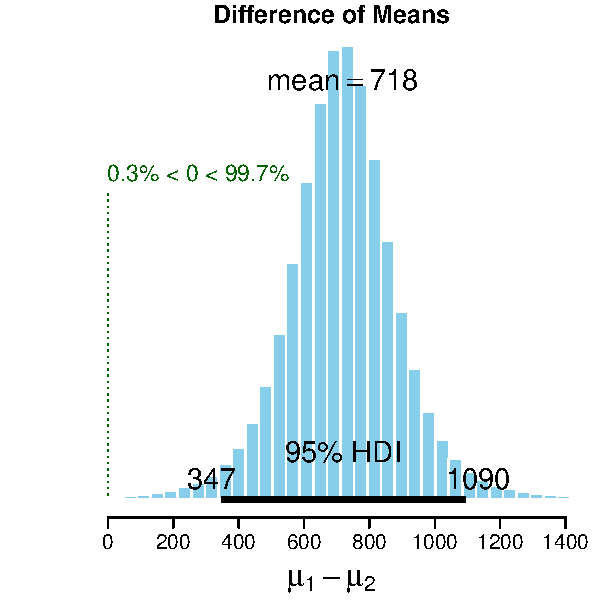
\includegraphics[width=.4\textwidth]{figures/cropped/tiff2pdf-m-uni-afl}
    }
    \subfloat[\listswf: Union vs.\ \fairfuzz]{%
        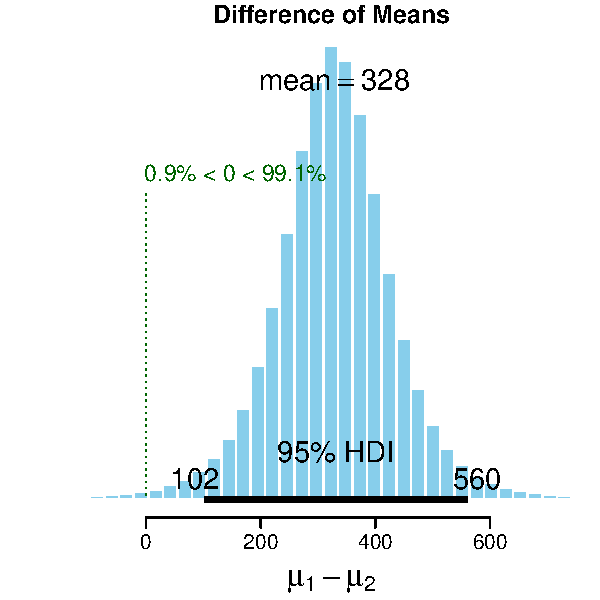
\includegraphics[width=.4\textwidth]{figures/cropped/ming-m-uni-fair}
    }
    \caption{Distribution of difference of means for union of fuzzers against
    the best single fuzzer.}
    \label{fig:means-mono-union}
\end{figure}

\section{Cooperative Fuzzing Evaluation}
\label{sec:eval-coop}

In this section we present an evaluation of the efficacy of cooperation.  For
this purpose we compare the results of running the \ac{CFF} for $6$ hours with
the union of coverage from the four fuzzers running without cooperation, as we
have done in Section~\ref{sec:eval-mono}. To make the comparison fair, for the
union we take the maximum coverage after $6$ hours. Table~\ref{tab:eval-coop}
presents the final mean coverage with $95\%$ confidence intervals.

\begin{table}[h]
    \centering%
    \begin{tabular}{l c c c}
        \textbf{\sut} & \textbf{multi} & \textbf{single} & \textbf{union} \\
        \bottomrule%
        \djpeg& $4056.4 \pm 76.9499$ & \hicell$4078.4 \pm 85.6738$ & $4028.6 \pm 47.7396$ \\
        \objdump& $5414.6 \pm 224.121$ & \hicell$5529.6 \pm 338.651$ & $5035.6 \pm 54.5944$ \\
        \tiffpdf& \hicell$8765.6 \pm 183.682$ & $8577.6 \pm 99.2457$ & $8623.2 \pm 183.399$ \\
        \listswf& \hicell$9008.4 \pm 122.81$ & $8801.4 \pm 96.4045$ & $8916.6 \pm 83.8381$
    \end{tabular}
    \caption{Mean coverage with $95\%$ confidence intervals for winning
    strategies that select single or multiple winners and without cooperation.}
    \label{tab:eval-coop}
\end{table}

Looking only at the final mean we can see that one of the two cooperative
strategies outperforms the union of fuzzers for all programs, but none of the
two outperforms the other. For \djpeg we see that the differences are too small
to be sensitive enough. By observing the mean coverage over time, shown in
Figure~\ref{fig:eval-coop-djpeg}, we see that the union of fuzzers struggles
against both cooperative strategies for the first two hours, before catching up.

\begin{figure}[h]
    \centering%
    \begin{adjustbox}{center}
        \subfloat[\djpeg]{%
            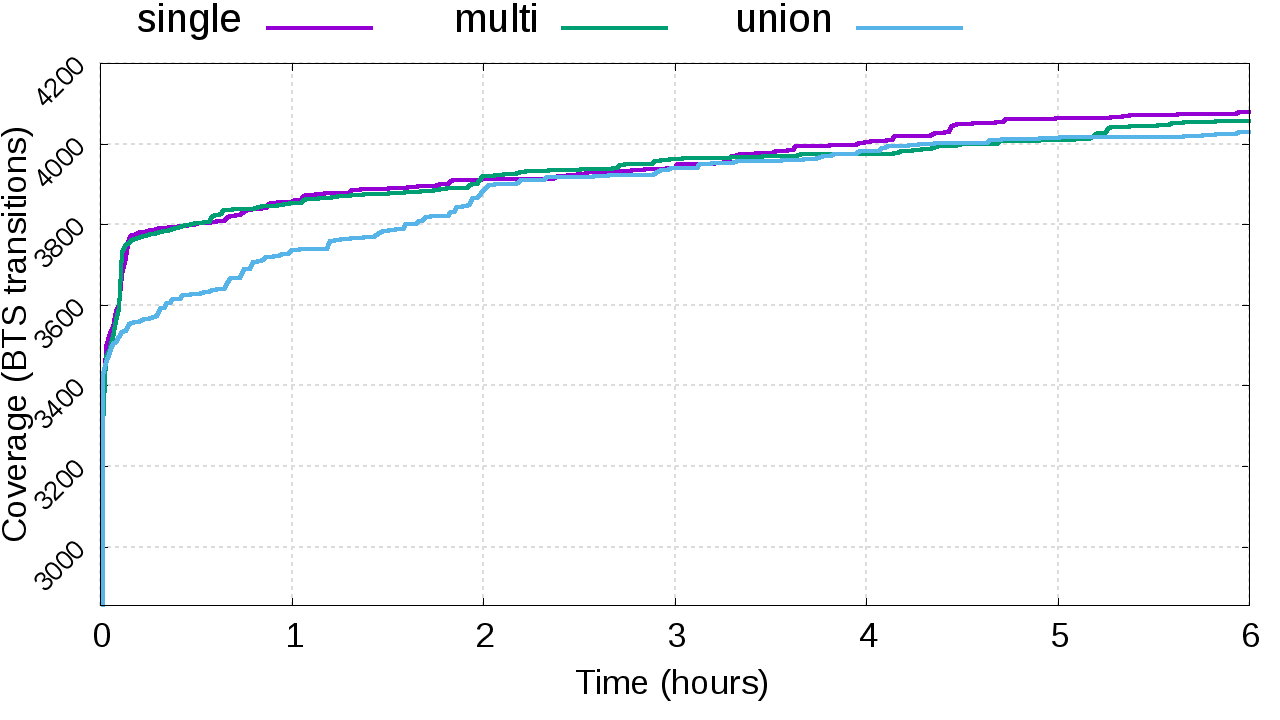
\includegraphics[width=.65\textwidth]{figures/vs-djpeg}
            \label{fig:eval-coop-djpeg}
        }
        \subfloat[\objdump]{%
            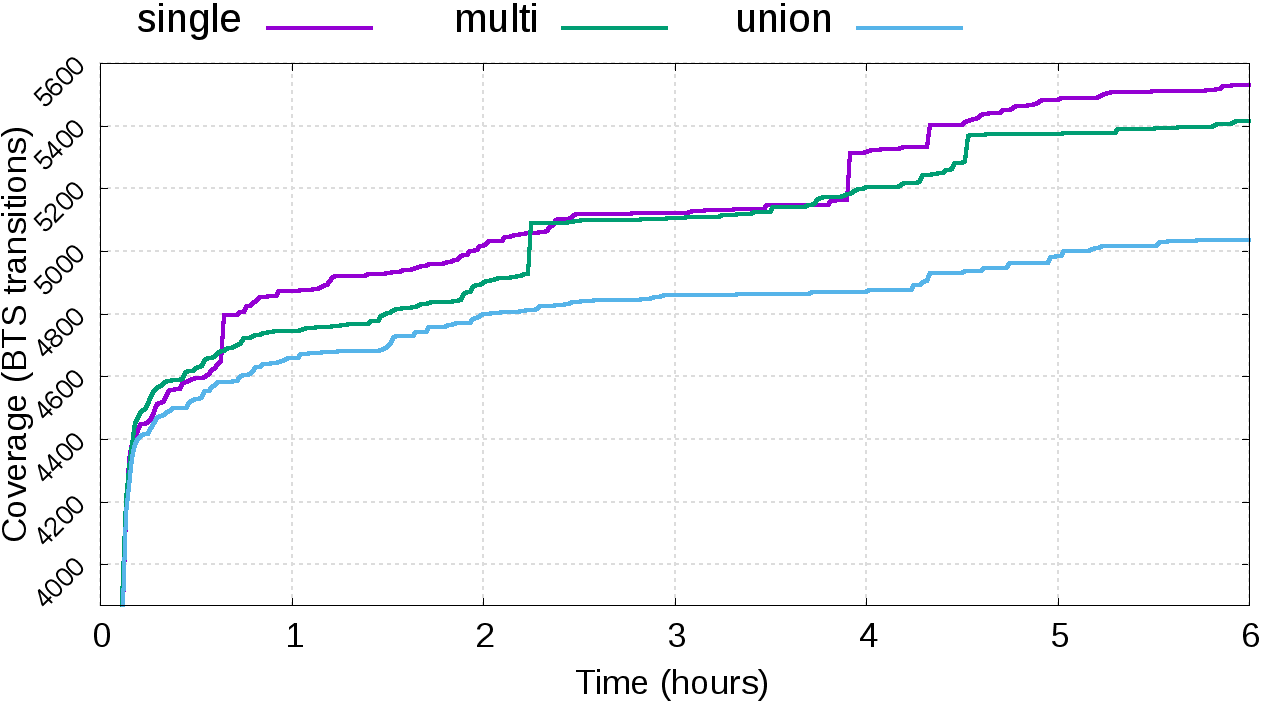
\includegraphics[width=.65\textwidth]{figures/vs-objdump}
            \label{fig:eval-coop-objdump}
        }
    \end{adjustbox}
    \begin{adjustbox}{center}
        \subfloat[\tiffpdf]{%
            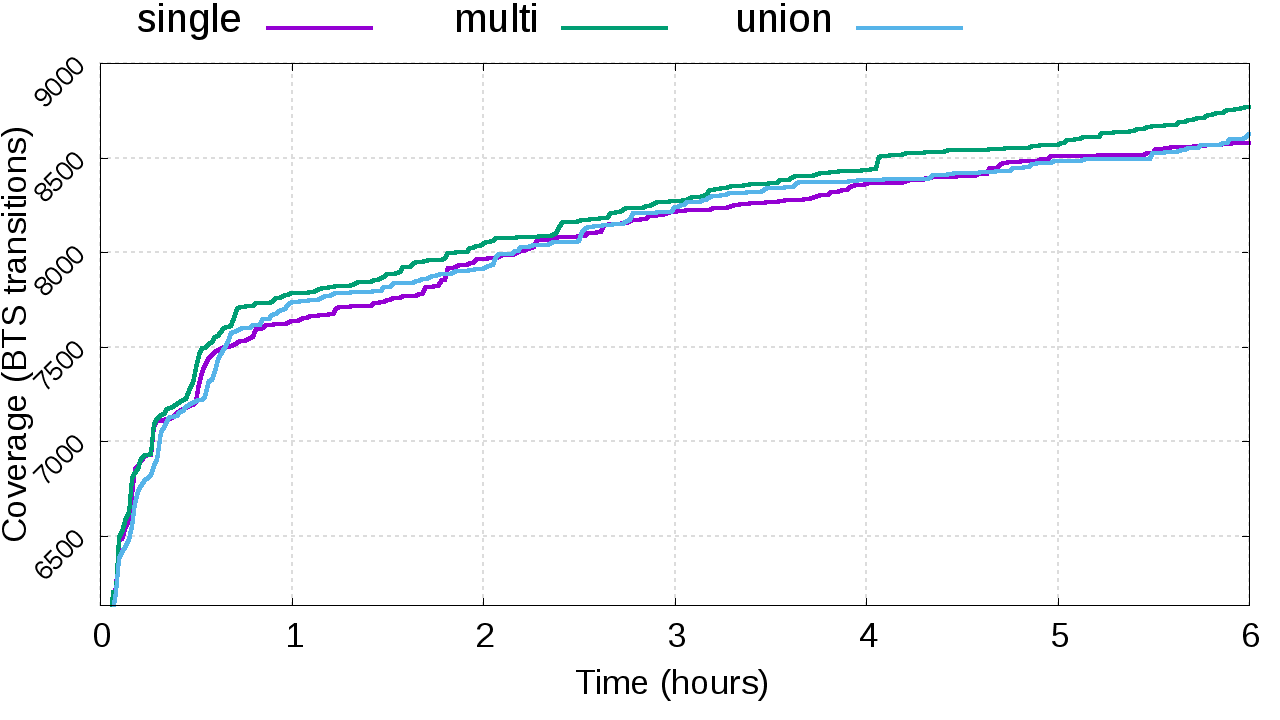
\includegraphics[width=.65\textwidth]{figures/vs-tiff2pdf}
            \label{fig:eval-coop-tiff2pdf}
        }
        \subfloat[\listswf]{%
            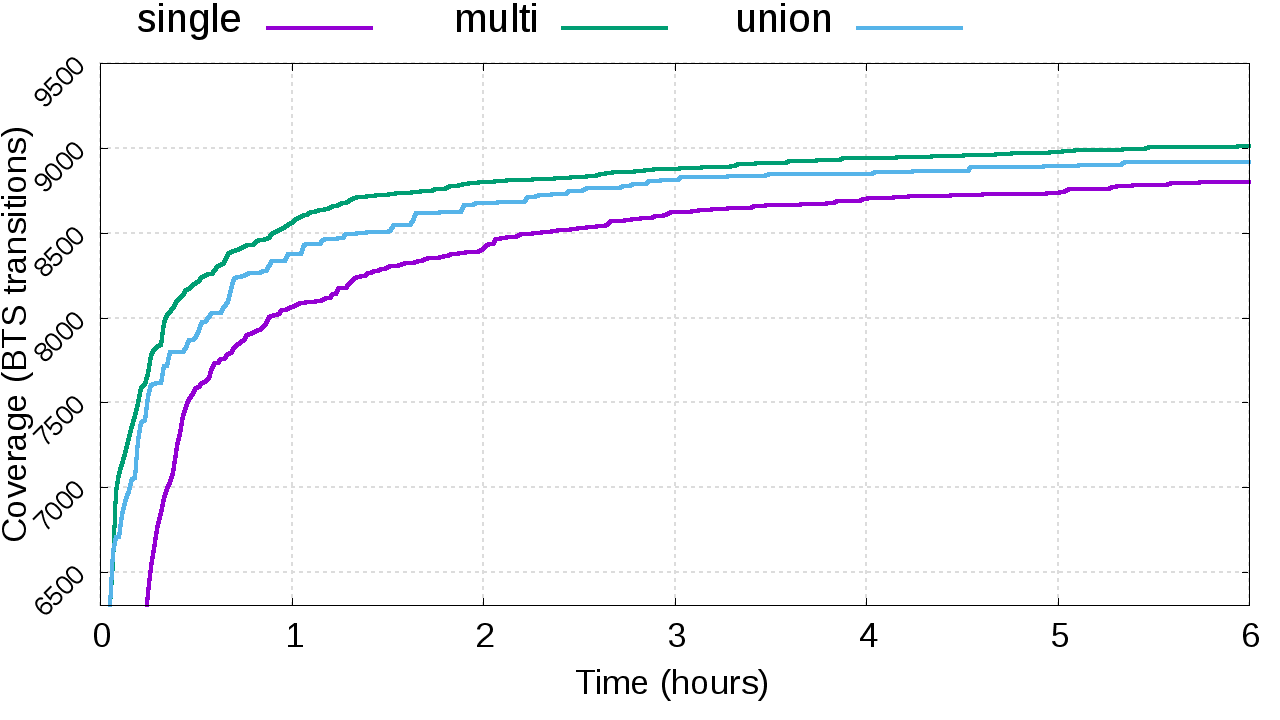
\includegraphics[width=.65\textwidth]{figures/vs-ming}
            \label{fig:eval-coop-ming}
        }
    \end{adjustbox}
    \caption{Mean coverage over time for two cooperative strategies and union of
    fuzzers.}
    \label{fig:eval-coop}
\end{figure}

\section{Crash Analysis}

